\documentclass[11pt]{article}
\usepackage[margin=0.91in,top=0.83in,bottom=0.85in]{geometry}
\usepackage{amsmath,amssymb,amsthm,booktabs,graphicx,xcolor,hyperref}
\definecolor{ink}{RGB}{24,51,73}
\hypersetup{colorlinks=true,linkcolor=ink,citecolor=ink,urlcolor=ink,pdftitle={Recovering prime powers and the modulus from three large prime sums}}
\newtheorem{theorem}{Theorem}
\newtheorem{lemma}[theorem]{Lemma}
\newtheorem{corollary}[theorem]{Corollary}
\newcommand{\dd}{\mathrm d}
\newcommand{\one}{\mathbf 1}
\newcommand{\R}{\mathbb R}
\newcommand{\C}{\mathbb C}
\newcommand{\Z}{\mathbb Z}
\newcommand{\Res}{\operatorname{Res}}
\newcommand{\e}{\mathrm e}
\newcommand{\re}{\operatorname{Re}}
\newcommand{\abs}[1]{\left|#1\right|}
\setlength{\emergencystretch}{1.6em}
\setlength{\parindent}{1.0em}
\begin{document}
\begin{center}
{\small\sffamily\color{ink} ANALYTIC NUMBER THEORY \quad / \quad RESEARCH NOTE}\par\vspace{11pt}
{\LARGE\bfseries Recovering prime powers and the modulus\\[4pt] from three large prime sums}\par\vspace{9pt}
{\large An extremal formula in arithmetic progressions}\par\vspace{7pt}
{\small 26 November 2026}
\end{center}
\begin{abstract}
Fix a modulus and take weighted prime counts at three cutoffs, $x$, $x\e^h$ and $x\e^{-h}$. We prove that the upper limit of their centered, square-root-normalized second difference, regarded as a function of $h>0$, has a slope jump at each detectable $h=\log p^k$. Its size recovers $\log p/\sqrt{p^k}$ and its location among the reduced residue classes obeys an explicit splitting law at primes dividing the modulus. The same profile is obtained with $x$ restricted to powers of two, even after any fixed initial segment of the prime data has been erased and the counts recentered. The square root of this profile defines a metric that determines the modulus up to the equivalence of an odd modulus and its double. Conversely, without invoking GRH, the growth exponent of the same statistic at any two distinct positive lags determines the supremum of the real parts of zeros.
\end{abstract}
\section{The arithmetic observable}
Let $q\ge1$, $G_q=(\Z/q\Z)^\times$, and $d=\varphi(q)$. For $q=1$ use the one-element group. Write $\Lambda(p^k)=\log p$ for primes $p$ and $k\ge1$, and $\Lambda(n)=0$ otherwise. For $a\in G_q$ and real $x\ge1$ put
\begin{align}
 A_a(x)&=\sum_{\substack{n\le x\\ n\equiv a\pmod q}}\Lambda(n)\left(\frac1n-\frac1x\right),
 &c_a&=\lim_{x\to\infty}\left(A_a(x)-\frac{\log x}{d}\right),\label{eq:obs}\\
 Y_a(t)&=\e^{t/2}\left(A_a(\e^t)-\frac{t}{d}-c_a\right),
 &t&\ge0.\nonumber
\end{align}
The limit exists already by the classical fixed-modulus prime number theorem with its usual error term. An explicit expression appears in Section~\ref{sec:ramp}. The convention at a cutoff $n=x$ is immaterial because its weight vanishes. Define
\begin{equation}
 B_{a,h}(t)=2Y_1(t)-Y_a(t+h)-Y_{a^{-1}}(t-h),\qquad
 F_q(a,h)=\limsup_{t\to\infty} B_{a,h}(t).                 \label{eq:B}
\end{equation}
Here $t\ge |h|$. The three terms are computed from the same prime table. Each is normalized at its own cutoff. The inverse residue in the last term is essential for the nonnegative multiplier in the proof.

\section{The recovery theorem}
For $n=p^k$ let $v=v_p(q)$ and $m=q/p^v$, including $v=0$. Define a probability distribution on $G_q$ by
\begin{equation}
 P_q(a;p^k)=\frac{\one_{\{a\equiv p^k\ (\mathrm{mod}\ m)\}}}{\varphi(p^v)} .       \label{eq:P}
\end{equation}
When $p\nmid q$ this puts all the mass at $p^k\bmod q$. If $p\mid q$, it fixes the residue modulo $m$ and gives equal mass to each lift across the $p$-part of $q$.

\begin{theorem}[Prime-power recovery]\label{th:main}
For $a\in G_q$, $F_q(a,h)$ is finite and nonnegative for all real $h$. On $h>0$ it is continuous and real analytic off the logarithms of prime powers. At any integer $n>1$ its right derivative minus its left derivative is
\begin{equation}
 F_q'(a,\log n+)-F_q'(a,\log n-)=
 \begin{cases}
 -\dfrac{2\log p}{\sqrt{p^k}}P_q(a;p^k),&n=p^k,\\[4pt]
 0,& n\text{ has at least two distinct prime factors}.
 \end{cases}                                                   \label{eq:jump}
\end{equation}
If the displayed weight is zero, the function is analytic at that point. The same $F_q$ results if the centers $x=\e^t$ are restricted to $b^j$, $j\in\mathbb N$, for any fixed $b>1$. For each $b$ there is a single sequence $j_\ell\to\infty$ realizing every one of these upper limits, for all moduli and residues and uniformly on any bounded interval of lags for each fixed modulus.
\end{theorem}

For example, no reduced residue class modulo $12$ contains $2$, yet the large-cutoff profiles for both $5$ and $11$ detect it. The entries below give $P_{12}(a;n)$, so each row is multiplied by $-2\log p/\sqrt n$ to obtain the actual jumps.
\begin{center}
\begin{tabular}{rcccc}
\toprule
$n$ & $a=1$ & $a=5$ & $a=7$ & $a=11$\\
\midrule
2 & 0 & $1/2$ & 0 & $1/2$\\
3 & 0 & 0 & $1/2$ & $1/2$\\
4 & $1/2$ & 0 & $1/2$ & 0\\
5 & 0 & 1 & 0 & 0\\
\bottomrule
\end{tabular}
\end{center}
Consequently $-\sqrt n/2$ times the sum of the slope jumps over $a$ is exactly $\Lambda(n)$. This is an identity of infinite limiting profiles. The order of operations is first the large-center upper limit at a fixed lag and then the one-sided derivatives in that lag.

\section{The prime remainder in the Lean proof}
The source file \texttt{PrimeError.lean} in Sernau's shorter edition of the Alp\"oge proof studies a smoothed sum with precisely the weight $1/n-1/x$. Its summand also carries the factor $1-\chi_K(n)$ and the restriction $n\equiv1\pmod q$. The residue of its transform involves a \emph{difference} of two families' zero multiplicities, divided by $\varphi(q)s(1-s)$. The development constructs short forms, proves that sufficiently many forms are available, and gives a lower bound on the sizes of integral forms. Their comparison produces a one-sided bound on that prime remainder and thence right-half-plane nonvanishing \cite{repo}. Here we retain the smoothing and allow the residue class to vary. Character orthogonality then gives a positive squared modulus after the three translations in \eqref{eq:B}.

The encyclopedia overview \cite{wiki} relates the critical line to prime-counting errors and describes the formal proof. For the exact scope we use the five statements in \texttt{grh/src/Main.lean}. In particular, for each Dirichlet character every open-strip zero is on the critical line. The independent checks of the shortened development compare the statements with the Mathlib challenge and check the proof terms \cite{verify}. We use the Dirichlet theorem at this point in the argument. The deductions below are proved in this note, in ordinary mathematics.

\section{The weighted explicit formula}\label{sec:ramp}
Write $\chi^*$ for the primitive character inducing $\chi\bmod q$, using $\zeta$ for conductor one. Define
\[
 D_a(s)=\frac1d\sum_{\chi\bmod q}\overline{\chi(a)}
        \left(-\frac{L'}L(s,\chi)\right)
       =\sum_{n\equiv a\, (q)}\frac{\Lambda(n)}{n^s}\qquad(\re s>1).
\]
If $D_a(1+w)=1/(dw)+b_a+O(w)$, then $c_a=b_a-1/d$. Indeed the pole at $s=1$ in the integral below contributes $(\log x)/d+b_a-1/d$. Equivalently partial summation gives $A_a(x)=\int_1^x\psi_a(u)u^{-2}\dd u$, where $\psi_a(u)=\sum_{n\le u,\, n\equiv a(q)}\Lambda(n)$. The fixed-$q$ prime number theorem makes the centered integral convergent and yields the same finite part. Explicitly,
\[
 c_a=\frac1d\left(-1-\gamma_E-\sum_{p\mid q}\frac{\log p}{p-1}
   -\sum_{\chi\ne\chi_0}\overline{\chi(a)}\frac{L'}L(1,\chi)\right).
\]

\begin{lemma}\label{lem:ramp}
Let $Z_\chi$ be the multiset of open-strip zeros of $L(s,\chi^*)$. With $x=\e^t$, as $t\to\infty$,
\begin{equation}
Y_a(t)=\frac1d\sum_{\chi\bmod q}\overline{\chi(a)}
   \sum_{\rho\in Z_\chi}\frac{\e^{(\rho-1/2)t}}{\rho(1-\rho)}
  +O_q((1+t)\e^{-t/2}).\label{eq:asym}
\end{equation}
This expansion also holds before using GRH. For a single primitive character the difference between its normalized sum and its displayed zero series is real analytic as a function of real $t>0$ (complex values are allowed).
\end{lemma}
\begin{proof}
For a primitive character $\xi$, apply Mellin inversion on $\re s=2$ to its prime sum. The integral is
\begin{equation}
 \frac{1}{2\pi i}\int_{2-i\infty}^{2+i\infty}
 -\frac{L'}L(s,\xi)\frac{x^{s-1}}{s(s-1)}\,\dd s .\label{eq:mellin}
\end{equation}
Indeed the two poles $0,1$ of the bare kernel give $1/n-1/x$ for $n<x$ and zero for $n>x$. At $n=x$ the values agree. In shifting the line left, the residue at a zero $\rho$ of multiplicity $r$ is $r x^{\rho-1}/[\rho(1-\rho)]$. The pole of the kernel at 1 gives a constant for nonprincipal $\xi$ and gives $\log x-1-\gamma_E$ for $\zeta$. At 0 we obtain $x^{-1}$ times a polynomial of degree at most one in $\log x$. A negative trivial zero at $-j$ contributes $-x^{-j-1}/[j(j+1)]$, for positive integers $j$ of the appropriate parity. This last series and each of its derivatives converge locally uniformly for $t>0$ and extend holomorphically to $\re t>0$.

For clarity, the standard contour estimates used here follow from the local zero count $O_q(\log(2+|T|))$ in a unit interval and the local partial fraction formula for $L'/L$ \cite{dav}. For each fixed left boundary $-J-1/2$, the horizontal sides can be taken at heights tending to $\pm\infty$ at distance $\gg_q 1/\log(2+|T|)$ from the neighboring ordinates. There $L'/L=O_{q,J}(\log^2(2+|T|))$ throughout the fixed strip, so the quadratic denominator kills the horizontal integrals. On the left edge the functional equation, reflection and Stirling formulas, and the absolutely convergent log derivative at $1-s$ bound $L'/L$ by $O_q(\log(2+J+|\Im s|))$ for $J\ge1$. Its integral tends to zero as $J\to\infty$ for each $x>1$. The zero count gives $\sum_\rho1/|\rho(1-\rho)|<\infty$; it also justifies the order of summation for fixed $t$ without GRH.

Passing from $\chi^*$ to $\chi$ removes terms at powers of primes dividing $q$ but absent from the conductor. Their partial sums of absolute weights are $O_q(1+\log x)$. After subtracting their convergent $1/n$-weighted constant, partial summation bounds the resulting normalized tail by $O_q((1+\log x)/\sqrt x)$. Averaging over characters yields \eqref{eq:asym}.
\end{proof}

\section{A sharp upper limit and its derivatives}
By Dirichlet GRH, write $\rho=1/2+i\gamma$ with $\gamma\in\R$. Define
\[
 K_q(a,u)=\frac1d\sum_{\chi\bmod q}\sum_{\rho\in Z_\chi}
       \frac{\overline{\chi(a)}\e^{i\gamma u}}{1/4+\gamma^2}.
\]
Absolute uniform convergence makes $K_q$ continuous. Conjugating the characters and zeros shows it is real. It satisfies $K_q(a^{-1},-u)=K_q(a,u)$. These facts include complex characters and central zeros, counted with their actual multiplicities.

\begin{proof}[Proof of Theorem \ref{th:main}]
In \eqref{eq:B} the coefficient multiplying $\e^{i\gamma t}/[d(1/4+\gamma^2)]$ is
\[
 2-\overline{\chi(a)}\e^{i\gamma h}-\chi(a)\e^{-i\gamma h}
       =|1-\overline{\chi(a)}\e^{i\gamma h}|^2 .
\]
It is real and lies in $[0,4]$. The triangle inequality bounds the upper limit by the sum of these nonnegative coefficients with their positive denominators. This bound is attained. Enumerate the ordinates for all Dirichlet characters, a countable set. For any first $N$ ordinates and $b>1$, the powers of $(\e^{i\gamma_1\log b},\ldots,\e^{i\gamma_N\log b})$ in the $N$-torus return arbitrarily near the identity at arbitrarily large positive indices. For example, take a convergent subsequence of powers with gaps tending to infinity and take quotients of consecutive terms. A diagonal sequence $j_\ell$ works for every ordinate. Absolute summability for each $q$ and the bound 4 give convergence of the series along $t=j_\ell\log b$, uniformly in $h$; the error in \eqref{eq:asym} tends uniformly to zero for bounded $h$. Thus
\begin{align}
 F_q(a,h)
 &=\frac1d\sum_{\chi,\rho}
   \frac{|1-\overline{\chi(a)}\e^{i\gamma h}|^2}{1/4+\gamma^2}
 =2\bigl(K_q(1,0)-K_q(a,h)\bigr).\label{eq:sharp}
\end{align}
No independence of zero ordinates enters this recurrence.

To compute a derivative jump at $h=\log n>0$, use the \emph{exact primitive} contour expansion in the proof of Lemma \ref{lem:ramp}. Its terms apart from the finite prime ramp and the zero series are analytic near $h$. One prime term in the normalized ramp is
\[
 \Lambda(n)\chi^*(n)\bigl(\e^{h/2}/n-\e^{-h/2}\bigr)\one_{h\ge\log n}.
\]
It is continuous and its derivative jumps by $\Lambda(n)\chi^*(n)/\sqrt n$. A locally finite sum of such terms is analytic between its active breakpoints. Thus the jump of $K_q'$ is the character average of these numbers. For $n=p^k$ the Chinese remainder theorem decomposes $G_q$ into $G_{p^v}\times G_m$. Only characters trivial on $G_{p^v}$ have primitive inducer nonzero at $p$. For those characters the value there is the character of $G_m$ evaluated at $p^k$. Orthogonality on $G_m$ gives
\[
 \frac1d\sum_{\chi}\overline{\chi(a)}\chi^*(p^k)
   =\frac{\varphi(m)}{d}\one_{a\equiv p^k\, (m)}=P_q(a;p^k).
\]
The same calculation includes $v=0$ and $m=1$. Zero average removes the entire local ramp. Multiplication by $-2$ in \eqref{eq:sharp} proves the derivative formula.
\end{proof}

\section{Recovering the modulus from distances alone}
Write $X_q=G_q\times\R$. For $u=(a,s)$ and $v=(b,t)$ set
\[
 D_q(u,v)=\sqrt{F_q(a^{-1}b,t-s)} .
\]
Thus all the distances can be defined directly from the prime sums. A stronger inverse question forgets even the names of the points. Could the same distances come from a different modulus?

\begin{theorem}[Rigidity of the modulus]\label{th:rigid}
$D_q$ is a metric. Put $q^\flat=q/2$ if $q\equiv2\pmod4$ and $q^\flat=q$ otherwise. Then
\[
 (X_q,D_q)\text{ is isometric to }(X_r,D_r)
 \quad\Longleftrightarrow\quad q^\flat=r^\flat.
\]
For fixed $q$, all surjective isometries are precisely
\[
 (a,t)\longmapsto(a_0a^\epsilon,b+\epsilon t),
 \qquad a_0\in G_q,\ b\in\R,\ \epsilon\in\{1,-1\}.
\]
\end{theorem}
For example, moduli $8$ and $12$ both have unit group isomorphic to $C_2\times C_2$. Their distances distinguish them. The primes $5$ and $13$ have the same residue modulo $8$ and different residues modulo $12$. In contrast, moduli $5$ and $10$ give identical distances under reduction.
\begin{proof}
\emph{Separation and the scale of a short interval.}
Formula \eqref{eq:sharp} realizes $D_q$ as Hilbert distance using coordinates
$\overline{\chi(a)}\e^{i\gamma t}/\sqrt{d(1/4+\gamma^2)}$. This gives the triangle inequality and translation invariance. For $0<u<\log 2$ there are no prime terms in the primitive contour expansion. At $a=1$, each character contributes to $K_q$ a function analytic at zero plus
\[
 \sum_{j>0\ {\rm trivial}}\frac{\e^{-(j+1/2)u}}{j(j+1)} .
\]
The notation selects even or odd positive $j$ according to parity. Twice differentiating the series gives the parity-geometric sum plus a bounded error, since $(j+1/2)^2/[j(j+1)]=1+1/[4j(j+1)]$. Each parity-geometric sum is $1/(2u)+O(1)$. Hence $\partial_uK_q(1,u)=\tfrac12\log u+O_q(1)$. Integration and continuity give
\begin{equation}
 r_q(u)^2:=F_q(1,u)=u\log(1/u)+O_q(u)\qquad(u\downarrow0).\label{eq:scale}
\end{equation}
A point at distance zero from the identity fixes every spectral coordinate. Its translation therefore preserves $K_q$. A nonzero time displacement would carry the unbounded one-sided slope at $(1,0)$ to a point with finite slopes, contradicting Theorem \ref{th:main} and inversion symmetry. With time displacement zero, the point must satisfy $\chi(a)=1$ for every $\chi$, since each primitive inducer has nontrivial zeros. Characters separate group elements. This proves separation.

\emph{Time lines and their parametrization.}
Choose a nonzero ordinate $\gamma_0$ of a zeta zero. The coordinate $\e^{i\gamma_0t}$ occurs with positive weight in the principal channel. Along any $D_q$-continuous path $s\mapsto(a(s),t(s))$ it admits a continuous real phase $v(s)$ with $\e^{iv(s)}=\e^{i\gamma_0t(s)}$. By \eqref{eq:sharp}, ordinary real time displacements give continuous paths, and the translation-invariant metric makes group operations continuous. Subtracting the time path $v(s)/\gamma_0$ leaves a continuous map into the countable metric subspace $G_q\times(2\pi/\gamma_0)\Z$. A connected subset of a countable metric space is a singleton, as otherwise distances from one of its points would fill a nondegenerate interval. Thus $a(s)$ is constant and $t(s)$ is ordinarily continuous. Conversely, every time line is path connected.

An isometry onto $X_r$ therefore acts by $(a,t)\mapsto(\sigma(a),f_a(t))$ for a bijection of the residues and ordinary homeomorphisms $f_a$ of $\R$ (apply the path argument also to the inverse). Set $g(y)=y^2/[2\log(1/y)]$ for small $y>0$. Equation \eqref{eq:scale} gives $g(r_q(u))/u\to1$ for every modulus. Since $r_r(|f_a(t+u)-f_a(t)|)=r_q(|u|)$, we obtain $|f_a(t+u)-f_a(t)|/|u|\to1$ at each $t$. Monotonicity and the mean value theorem give $f_a(t)=\epsilon_a t+b_a$ with $\epsilon_a=\pm1$.

\emph{Arithmetic identifies the relative origins.}
For any two lines the profile of their squared distance is nonconstant. Dirichlet's theorem supplies a prime in their quotient residue class, and \eqref{eq:jump} gives a nonzero jump there. If two lines had opposite orientations, translating both input times equally would hold the input distance fixed and sweep the entire target profile, a contradiction. After simultaneous inversion of residue and time in the target, which is an isometry by \eqref{eq:sharp}, we may assume every orientation positive.

Fix lines $a,b$. For each sufficiently large prime $p\equiv a^{-1}b\pmod q$, the target profile has a kink at $\log p+b_b-b_a>0$. Hence $Cp$ is an integer, where $C=\e^{b_b-b_a}$. Two distinct such primes and B\'ezout's identity give $C\in\Z$. Applying the same argument to the inverse between the image lines gives $C^{-1}\in\Z$. Thus all the $b_a$ are equal. Compose with a common time and residue translation to fix $(1,0)$. For every prime $p\nmid qr$, its positive kink now forces
\[
 \sigma(p\bmod q)=p\bmod r .
\]
For $q=r$ this fixes every residue, proving the isometry description after undoing the normalizations. Every map in the statement is indeed an isometry.

For general $q,r$, let $L=\operatorname{lcm}(q,r)$. Every unit modulo $L$ contains a prime. The last identity implies $\sigma\pi_q=\pi_r$ for the reduction maps on $G_L$, so their kernels agree. Restricting to the local factor $G_{p^{v_p(L)}}$ in the Chinese remainder decomposition gives $\varphi(p^{v_p(q)})=\varphi(p^{v_p(r)})$. For odd $p$ these values strictly increase with the exponent starting at zero. For $p=2$ only exponents zero and one coincide. This proves necessity. Conversely, for odd $m$, reduction $G_{2m}\to G_m$ is an isomorphism. Its character bijection preserves primitive inducers and every term in \eqref{eq:sharp}. This gives the asserted isometry, including $m=1$.
\end{proof}

\section{A converse with two fixed lags}
The same arithmetic observable detects the edge of the zero set, an assertion that can be proved without first placing any zeros on the critical line. Denote by $\Theta_q$ the supremum of $\re\rho$ over all $Z_\chi$ for $\chi\bmod q$. Functional-equation symmetry gives $\Theta_q\ge1/2$.
\begin{theorem}\label{th:two}
For every $a\in G_q$ and $0<h_1<h_2$,
\[
 \limsup_{t\to\infty}\frac1t\log\left(1+\max_{j=1,2}|B_{a,h_j}(t)|\right)
     =\Theta_q-\tfrac12 .
\]
In particular, boundedness of both functions on a tail of the real time axis is equivalent to Dirichlet GRH at modulus $q$.
\end{theorem}
\begin{proof}
Absolute summability in \eqref{eq:asym} bounds each shifted function by $O_{q,h}(\e^{(\Theta_q-1/2)t})$ for large $t$. For the reverse inequality, write $z=s-1/2$. Direct integration on $\re z>1/2$ gives
\[
 \int_0^\infty Y_a(t)\e^{-zt}\dd t
   =\frac{D_a(s)}{s(s-1)}-\frac{1/d}{(s-1)^2}-\frac{c_a}{s-1}.
\]
At a zero $\rho$ with $\eta=\re\rho-1/2>0$, let $m_\chi$ be its multiplicity for $\chi^*$ and $M=\sum m_\chi>0$, $C=\sum m_\chi\overline{\chi(a)}$. Put $z_0=\rho-1/2=\eta+i\gamma$. A time shift by $u$ multiplies the transform by $\e^{zu}$ up to an entire correction when all integrals are taken on a common tail $t\ge h_2$. Thus at $z_0$ the residue of the transform of $B_{a,h}$ equals
\[
 \frac{H(h)}{d\rho(1-\rho)},\qquad
 H(h)=2M-\e^{z_0h}C-\e^{-z_0h}\overline C.
\]
The imprimitive Euler factors have no zeros with $\re\rho>1/2$. Write $s_0=|C|/M\le1$, $u=\eta h$, and $c=\cos(\arg C+\gamma h)$ if $C\ne0$. Then
\[
 \frac{|H(h)|^2}{4M^2}
 =1-2s_0\cosh(u)c+s_0^2(\sinh^2(u)+c^2)
 \ \ge\ (1-s_0\cosh u)^2.
\]
The quadratic is decreasing for $-1\le c\le1$, and the bound holds also for $C=0$. If $A=\cosh(\eta h_1)$ and $B=\cosh(\eta h_2)$, then
$\max(|1-s_0 A|,|1-s_0 B|)\ge (B-A)/(B+A)$, by taking $B(1-s_0 A)-A(1-s_0 B)$. Hence at least one transform has a genuine pole. If the limsup exponent were less than $\eta$, absolute convergence would make both transforms holomorphic near $z_0$. Taking the supremum over the zeros proves the lower bound when $\Theta_q>1/2$; at $\Theta_q=1/2$ nonnegativity suffices. In this latter case \eqref{eq:asym} gives actual boundedness. Reflection of strip zeros about the critical line gives the equivalence.
\end{proof}

\section{Erasing data and checking the scalar case}
The limiting profile recovers small prime powers even if their entries have been removed from the input prime table. More generally, in each class perturb the weights by numbers whose running sum $E(u)$ is $o(\sqrt u)$. The change in $A_a(x)$ is $\int_1^x E(u)u^{-2}\dd u$ for weights indexed by $n\ge1$, with the same formula at $n=1$. Recompute $c_a$ by \eqref{eq:obs}. The resulting change in $Y_a(\log x)$ is
\[
 -\sqrt{x}\int_x^\infty E(u)u^{-2}\dd u=o(1).
\]
Indeed its absolute value is at most $2\sup_{u\ge x}\bigl(|E(u)|/\sqrt u\bigr)$. Thus all three terms in \eqref{eq:B} retain their original limiting profile. This covers deletion of any finite initial segment.

For $q=1$ the check requires only finitely many prime powers at each $h>0$ and an elementary correction. With $K(h)=K_1(1,h)$,
\[
 K(h)=Y_1(h)-\e^{-h/2}\left(\log(2\pi)-
      \sum_{k\ge1}\frac{\e^{-2kh}}{2k(2k+1)}\right),
 \qquad K(0)=2+\gamma_E-\log(4\pi).
\]
These identities follow from \eqref{eq:mellin}, using $\zeta'(0)/\zeta(0)=\log(2\pi)$, and continuity at zero. The script checks one-sided differences at $\log 2,\log 4,\log 6$ at 72-decimal-digit working precision, and separately evaluates the primitive-character average for all prime powers up to 250 modulo 12. For instance the slopes at $\log2$ are approximately $0.450030537632177$ and $-0.530227605836371$; their difference agrees with $-2\log(2)/\sqrt2$. These calculations test the formulas. Their proofs are given above.
\begin{figure}[htbp]
\centering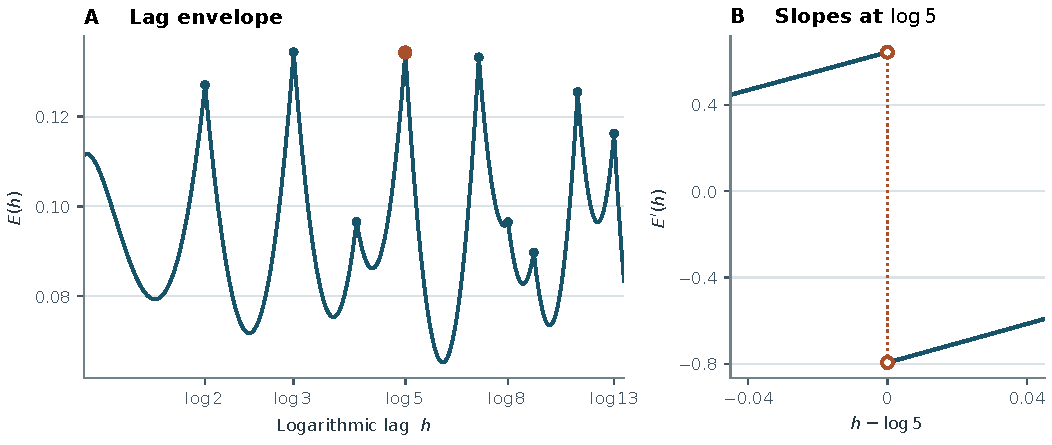
\includegraphics[width=\linewidth]{lag_profile.pdf}
\caption{The limiting profile computed from the finite prime sum at modulus one. The magnified derivative has a jump of $-2\log(5)/\sqrt5$ at the marked lag.}
\end{figure}

\clearpage
\section{Relation to earlier work and further questions}
Nicolas uses the scalar zero series with denominator $\rho(1-\rho)$ \cite{nicolas}. Akbary and Francis use simultaneous approximation to attain an unshifted extremum for a related character sum \cite{af}. Suzuki's screw functions contain linear ramps on the prime side and reciprocal-square zero weights on the spectral side \cite{suzuki,suzuki2}. Chirre, Pereira J\'unior and de Laat develop a progression version of the Guinand--Weil explicit formula \cite{cpd}. These precedents account for the scalar kernel, recurrence mechanism and prime-power singularities. The contributions proposed here are the three-cutoff extremal identity with residue labels, its classification of the unlabelled metric spaces, and the quantitative two-lag protection against cancellation at a shared zero. A targeted literature search found no earlier statement of these combined results. Historical priority remains open to further bibliography.

Two questions concern the cost of recovery. How large a dyadic center suffices to approximate the entire lag profile within $\varepsilon$ on a prescribed interval? How accurately do a finite set of noisy distances and a bounded range of lags distinguish two moduli? The proofs here use arbitrarily large centers for recurrence and exact distances for rigidity.
\begin{thebibliography}{9}\small
\bibitem{repo} L. Sernau et al., \emph{GRH for Dirichlet $L$-functions, in Lean 4}, commit \texttt{72fead102f66}, 25 November 2026. \href{https://github.com/lsernau/grh-lean/tree/72fead102f663d5c7a407964a13dc0cf9d977207}{Repository}; \href{https://github.com/lsernau/grh-lean/blob/72fead102f663d5c7a407964a13dc0cf9d977207/grh/src/New/Reduction/Zeros/PrimeError.lean}{weighted prime remainder}; \href{https://github.com/lsernau/grh-lean/blob/72fead102f663d5c7a407964a13dc0cf9d977207/grh/src/Main.lean}{exported statements}.
\bibitem{wiki} Wikipedia contributors, \href{https://en.wikipedia.org/wiki/Riemann_hypothesis}{\emph{Riemann hypothesis}}, accessed 26 November 2026.
\bibitem{verify} A. Sutherland, \href{https://math.mit.edu/~drew/shortgrh/}{\emph{Shorter Lean proof of RH and GRH for Dirichlet $L$-functions: verification files}}. See also \href{https://www.math.uwaterloo.ca/~mrubinst/alpoge_claude_grh/}{M. Rubinstein's verification records}.
\bibitem{dav} H. Davenport, \emph{Multiplicative Number Theory}, third edition, revised by H. L. Montgomery, Springer, 2000. See the chapters on zeros and the explicit formula.
\bibitem{nicolas} J.-L. Nicolas, \href{https://doi.org/10.4064/aa155-3-7}{Small values of the Euler function and the Riemann hypothesis}, Acta Arith. 155 (2012), 311--321, eqs. (1.3), (1.18).
\bibitem{af} A. Akbary and F. J. Francis, \href{https://arxiv.org/abs/1810.11524}{Euler's function on products of primes in progressions}, especially Remark 1.23(i).
\bibitem{suzuki} M. Suzuki, \href{https://doi.org/10.1112/jlms.12785}{Aspects of the screw function corresponding to the Riemann zeta-function}, J. Lond. Math. Soc. 108 (2023), 1448--1487.
\bibitem{suzuki2} M. Suzuki, \href{https://arxiv.org/abs/2209.12832}{Screw functions of Dirichlet series in the extended Selberg class}, Int. J. Number Theory 21 (2025), 1815--1823.
\bibitem{cpd} A. Chirre, V. J. Pereira J\'unior and D. de Laat, \href{https://arxiv.org/abs/2005.02393}{Primes in arithmetic progressions and semidefinite programming}, arXiv:2005.02393.
\end{thebibliography}
\end{document}
